%todo:
% - edit abstract
% - for exp. 2, plain mean doesn't differ from DD 
% %%% finish expt 2 results: update correlation and report split-half correlation. show that the means differ across contexts.

% - get tiny URLs for experiment links
% - set up forest page

% - fit into space and proof read.
% - if time: look at "order effect" in prior elicitation (taboo sampling hypothesis... first sample is 0, second is 100, third - fifth are meh)

% - make figures 1 & 2 as pretty as 3 & 4


%noah's todo:
% - make it more clear why we do the fully-fixed-semantics model, possibly shorten that section if there's not space.
% - add a bit more sign-posting as to why we're doing the various fancy BDAs.


% - try rationality parameter in tfbt model
% - look at "order effect" in prior elicitation (taboo sampling hypothesis... first sample is 0, second is 100, third - fifth are meh)
% - do we really want posterior predictives that include the guessing parameter? (the guessing parameter is part of the analysis model, not the cognitive model...)
%- what kind of evidence do we want to use at the end to relate inferred priors to elicited? 
%	- is eye-balling the elicited prior and the mean inferred priors sufficient?
%	- i tried TFBT on the elicited priors to back out gamma & deltas, but gammas don't seem to come apart for DD vs. plain (as they do in the inferred priors from Exp 1 &2)
%	- one possible way to get this sort of "ordered gammas" evidence would be to repeat the prior elicitation with more items per trial
%		- the thought is that in our prior elicitation, i used 5 animals per slide (and 6 trials)
%			- probably there was not enough dynamic range for Plain vs DD to come apart 
%		- i think with 10 items, it would be better (but does that mean just 3 trials, one in each context, per subj?) [there are only 30 animals]
%% --- not sure if the above comments about prior elicitation still hold with the fixed TFBT model, but Noah's suggestion was for 1 animal at a time

%		
%todo after cogsci:
%-run additional contexts. e.g. separate dangerous and distinct.
%-look again at finer-grained truth judgement task?
%-think about the weird cases of generics in the literature. e.g. ``robins lay eggs''.
% - try an S2 model of prevalence judgement task, too. does it reduce to the L1 model?

%




\documentclass[10pt,letterpaper]{article}

\usepackage{cogsci}
\usepackage{pslatex}
\usepackage{apacite}
\usepackage{url}
\usepackage{graphicx}
\usepackage{caption}
\usepackage{subcaption}
\usepackage{listings}
\usepackage{color}
\usepackage{textcomp}
\usepackage{amsmath}
\usepackage{amssymb}
\usepackage{wrapfig}

\graphicspath{{figures/}}

\def\signed #1{{\leavevmode\unskip\nobreak\hfil\penalty50\hskip2em
  \hbox{}\nobreak\hfil(#1)%
  \parfillskip=0pt \finalhyphendemerits=0 \endgraf}}

\newsavebox\mybox
\newenvironment{aquote}[1]
  {\savebox\mybox{#1}\begin{quote}}
  {\signed{\usebox\mybox}\end{quote}}


\lstset{
  language=Scheme, % Andreas Stuhlmuller. Scheme listings. https://github.com/stuhlmueller/scheme-listings.git
  columns=fixed,
  tabsize=2,
  extendedchars=true,
  breaklines=true,
  frame=single,
%  numbers=left,
  numbersep=5pt,
   basicstyle=\scriptsize\ttfamily
%  rulesepcolor=\color{solarized@base03},
%  numberstyle=\tiny\color{solarized@base01},
%  keywordstyle=\color{solarized@green},
%  stringstyle=\color{solarized@cyan}\ttfamily,
%  identifierstyle=\color{blue},
%  commentstyle=\color{solarized@base01},
%  emphstyle=\color{solarized@red}
}

\definecolor{Red}{RGB}{255,0,0}
\newcommand{\red}[1]{\textcolor{Red}{#1}}  


\title{Words are vague: A model of generic language}
 
% \author{{\large \bf Michael Henry Tessler, Noah D. Goodman } \\
%	\{mhtessler, ngoodman\}@stanford.edu \\
%  Department of Psychology, Stanford University}

\author{{\large \bf Michael Henry Tessler} (mhtessler@stanford.edu), {\large \bf Noah D. Goodman} (ngoodman@stanford.edu) \\
  Department of Psychology, Stanford University}

 
\begin{document}
\maketitle


\begin{abstract}
Generic utterances are ubiquitous in natural language. Despite their prevalence, the meanings of generic statements are puzzling to formal approaches. \citeA{Cimpian2010} demonstrated that generic statements can be endorsed with little evidence while the same sentences can be interpreted strongly. Here, we replicate this effect and investigate how well models of scalar semantics can account for this behavior. We use techniques from Bayesian data analysis to make inferences about the putative threshold used as well as to arbitrate between competing accounts. We show how a simple scalar semantics is untenable, but that the same semantics within a probabilistic pragmatics framework can account for the data. In this model, the generic has an underspecified semantics, but this uncertainty is resolved by context and interaction. The differences between verification and interpretation are understood as different tasks within a communicative framework. We use a Bayesian analysis again to infer a prior distribution, for which we then find confirmatory evidence in Exp. 2. We conclude with a couple of simulations about properties of particular theoretical interest. 

\textbf{Keywords:} 
generics; pragmatics; bayesian cognition; bayesian data analysis
\end{abstract}

\begin{aquote}{Barack Obama, \emph{2015 State of the Union Address}}
New sanctions passed by this Congress, at this moment in time, will all but guarantee that diplomacy fails -- alienating America from its allies; making it harder to maintain sanctions; and ensuring that Iran starts up its nuclear program again.
\end{aquote}


Generic meanings are hard to pin down.  Consider President Obama's remark during the State of the Union Address. The sentence is a generic statement about \emph{new sanctions} in that it conveys a generalization about the members of this kind \cite{Carlson1977, Leslie2008}. It invites the question: ``Exactly how many of these new sanctions will guarantee diplomatic failure?'' President Obama's statement is conceivably true if most or only a few new sanctions will be problematic. At the same time, he is not a man to waste words---why does he go through the trouble of producing such a vague utterance? In this paper, we will see that the \emph{context} in which his words are uttered contributes to the meaning we derive. We propose that this aspect of generic language follows from pragmatic reasoning about an uncertain threshold for meaning; an idea which we formalize in a probabilistic model within the Rational Speech Acts framework \cite{Frank2012,Goodman2013}.

Generic statements are puzzling because their meaning is so flexible. On the one hand, generics would seem to suggest an almost universal quantification, as in ``Dogs bark''. Others, like ``Mosquitos carry West Nile virus'', involve a property that applies only to a small subset of the kind. 
%It is perhaps this inherent uncertainty that leads generics to be so widespread in natural language. 
\citeA{Cimpian2010} (henceforth, CBG) carried out a series of experiments designed to examine the truth conditions and implications of generic statements. 
They found evidence for the influence of additional knowledge about a target property (e.g.~its \emph{distinctiveness}) on participants' willingness to accept generic statements---this type of contextual information modified the truth conditions. CBG also found an asymmetry between  interpretation and verification: in one task, participants interpreted a generic (e.g.~``lorches have purple feathers'') as nearly universal; in a different task, they would endorse the same generic as true at a much lower prevalence (``50\% of lorches have purple feathers'').

Both context and asymmetry effects pose a puzzle for the semantics of generics: what could be the stable meaning of a generic given this extreme flexibility? 
In this paper, we seek to explain both of these phenomena as the effects of pragmatic inference filling in a meaning that is underspecified in the semantics. 
In particular, we posit a scalar semantics for generics in which they express that \emph{prevalence}---the probability of the property given the kind---is above a threshold (cf. \citeA{Cohen1999}). Following \citeA{Lassiter2015}, we treat this threshold as a free variable that is reasoned about by a pragmatic listener: what is the threshold likely to be, given that a speaker bothered to utter the generic? Context effects follow from differences in prior beliefs about the distribution of the property across categories. Asymmetry effects follow by modeling differences in the language understanding and answer-selection task faced by participants in the different experiments (cf. \citeA{Degen2014}).  %suggested that different dependent measures in experimental pragmatics paradigms map onto different communicative roles, and thus should be modeled accordingly. 

%We draw on new advances in probabilistic pragmatics to formalize two possible theories of the generic. Further, we harness the power of Bayesian data analysis to mediate between these formal theories and draw inferences about cognitively interesting model parameters. 

In what follows, we first replicate the main effects reported by CBG, using Bayesian data analytic techniques to further examine the effective truth-conditions of generic statements. We then introduce a model of generic comprehension, within the probabilistic Rational Speech Acts framework. We show that this model predicts both context and asymmetry effects, given appropriate prevalence priors. Finally we experimentally elicit the prevalence priors in CBG's experimental contexts, verifying the predictions of the model.


%(e.g. ``These feathers are as sharp as needles and can easily get lodged in you, causing massive bleeding. No other animals have these kinds of feathers'')
% (e.g.  ``These feathers are wide and very smooth to the touch. Other animals have these kinds of feathers.'')

%How are we to understand these data? One interpretation is that context changes the truth-conditions for a generic statement, but that within a context, the truth-conditions are stable. A different sort of explanation is that context changes the nature of world somehow, and that generic meanings are inferred rationally from context. We draw on recent advances in probabilistic pragmatics and Bayesian data analysis to mediate between these two alternatives.


\section{Experiment 1: CBG replication}

In CBG's \emph{truth conditions} task, participants were given an evidence statement consisting of the percentage of a category that had a property (e.g. ``30\% of lorches have purple feathers''). Participants were asked whether the associated generic statement (i.e. ``Lorches have purple feathers'') was true or false. 

The authors manipulated context within-subjects by adding additional statements about the property. We focus on three contexts in this paper: \emph{dangerous and distinct} (DD, e.g.~``These feathers are as sharp as needles and can easily get lodged in you, causing massive bleeding. No other animals have these kinds of feathers''), \emph{not distinct and irrelevant} (NI, e.g.~``These feathers are wide and very smooth to the touch. Other animals have these kinds of feathers.''), and \emph{plain} (P, no additional statements). CBG found that DD increased the overall proportion of ``true'' responses of the generic propositions. 
%That is, when the property in question was dangerous and distinct, participants required a lower overall prevalence (e.g. 10\% of lorches had purple feathers) to assert that the generic statement was true.

In their \emph{implied prevalence} task, participants were supplied with the generic (again with context as a within-subjects variable) and asked to judge prevalence: ``What percentage of lorches do you think have purple feathers?''. CBG found that the generic was interpreted strongly---nearly all lorches have purple feathers---in all contexts. 

Experiment 1 attempted to replicate the main findings of CBG: that context affects the proportion of ``true'' responses to a generic statement (Exp. 1a) and that there is an asymmetry between interpretation and verification of the truth conditions of the generic (Exp. 1b). 
Exp. 1a and 1b were conducted on separate sessions, one week apart. None of the participants completed both experiments.

\subsection{Experiment 1a: \emph{truth conditions}}

\subsubsection{Participants}

We recruited 40 participants over Amazon's crowd-sourcing platform Mechanical Turk.  
%NDG: restrictions on IP address or native language?

\subsubsection{Procedure and materials}

Our procedure was very similar to CBG's \emph{truth conditions} task. Our instructions were elaborated to improve interest and motivation\footnote{The experiment in full can be viewed at \url{http://stanford.edu/~mtessler/experiments/generics/cbg2010-replication/experiment/experiment-9.html}}. 

We used the same materials as CBG (available in their Appendix). The materials used were 30 novel animals (e.g. lorches, morseths, blins) each paired with a unique property. Properties were pairs of colors and body-parts (e.g. purple feathers, orange tails). Each participant saw 30 unique animal-property pairs: 10 in each of 3 contexts (\emph{DD}, \emph{NI}, \emph{plain}). The 10 items in each context were randomly paired with 1 of 5 ``prevalence levels'': \{10, 30, 50, 70, 90\}\%; each prevalence level appeared 2 times per context. 

Participants saw a prevalence statement and a context statement (\emph{plain}, \emph{DD}, \emph{NI}, as illustrated above). 
%A context here was either (1) dangerous \& distinct statements (e.g. ``These feathers are as sharp as needles and can easily get lodged in you, causing massive bleeding. No other animals have these kinds of feathers.''), (2) not distinct \& irrelevant statements (e.g. ``These feathers are wide and very smooth to the touch. Other animals have these kinds of feathers.'', or (3) nothing else. 
Participants were then asked ``Is the following sentence true or false?'', below which was presented the associated generic (e.g. ``Lorches have purple feathers'') and true and false radio buttons. 

\subsubsection{Results}


\begin{figure}
        \centering
        \begin{subfigure}[b]{0.55\columnwidth}
                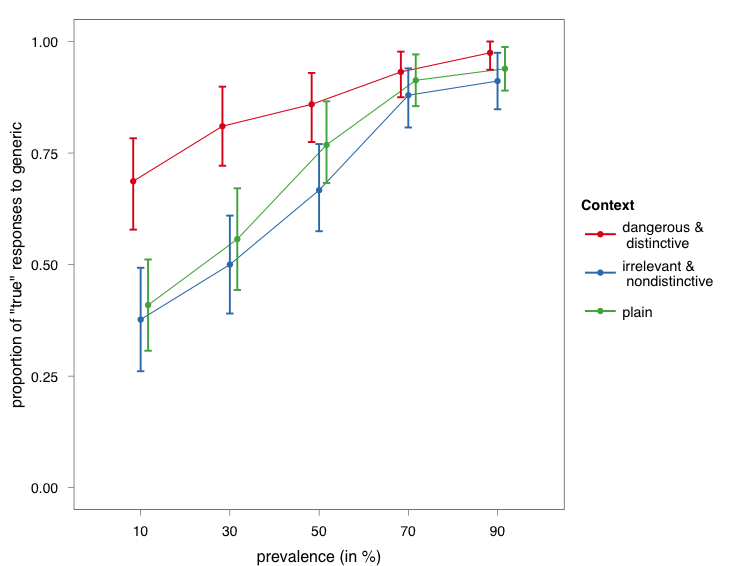
\includegraphics[width=\columnwidth]{data_truthconditions1}
                \caption{Truth conditions of the generic vary across contexts. Error bars denote bootstrapped 95\% confidence intervals.}
                \label{fig:datatc}
        \end{subfigure}%
        ~ %add desired spacing between images, e. g. ~, \quad, \qquad, \hfill etc.
          %(or a blank line to force the subfigure onto a new line)
        \begin{subfigure}[b]{0.45\columnwidth}
                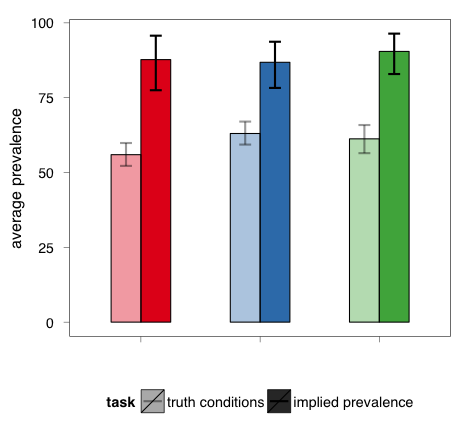
\includegraphics[width=\columnwidth]{data_asymmetry1}
                \caption{Asymmetry between verification and interpretation}
                \label{fig:datasym}
        \end{subfigure}
        ~ %add desired spacing between images, e. g. ~, \quad, \qquad, \hfill etc.
          %(or a blank line to force the subfigure onto a new line)
        \caption{Replication of CBG}\label{fig:exp1}
\end{figure}



%\begin{figure}
%\centering
%    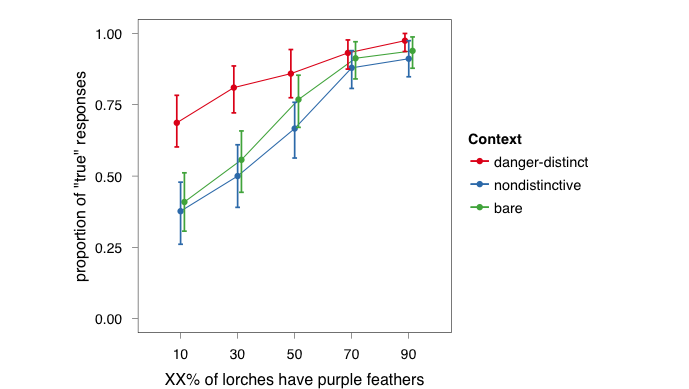
\includegraphics[width=\columnwidth]{fig1_replication}
%    \caption{Replication of CBG \emph{truth conditions}, generics condition}
%  \label{fig:replication}
%\end{figure}

Results are shown in Fig~\ref{fig:datatc}. We entered participant's truth judgments into a mixed effects logistic regression with random by-item and by-participant effects of intercept and fixed effects of prevalence and context as well as an interaction term.  Our results replicated the finding of CBG that the generic statement was endorsed more in the dangerous and distinctive (DD) context than in the plain (P) condition (Figure \ref{fig:datatc}; $z = 5.52; p < 0.001$). There was also an interaction between prevalence level and context such that the DD context was endorsed more than P at lower prevalence levels ($z=-2.353; p = 0.019$). There was a trending effect for the nondistinctive and irrelevant (NI) context to be endorsed \emph{less} than the plain context ($z=-1.91; p = 0.056$).

\subsection{Experiment 1b: \emph{implied prevalence}}

\subsubsection{Participants}

We recruited 30 participants over Amazon's crowd-sourcing platform Mechanical Turk.  

\subsubsection{Procedure and materials}

Our procedure was very similar to CBG's \emph{implied prevalence} task. Our instructions were elaborated to improve interest and motivation\footnote{The experiment in full can be viewed at \url{http://stanford.edu/~mtessler/experiments/generics/cbg2010-replication/experiment/experiment-12.html}}. 

The materials and context conditions were the same as in Exp. 1a. 
On each trial, participants saw a generic statement (instead of a prevalence statement) and a context. 
%A context here was either (1) dangerous \& distinct statements (e.g. ``These feathers are as sharp as needles and can easily get lodged in you, causing massive bleeding. No other animals have these kinds of feathers.''), (2) not distinct \& irrelevant statements (e.g. ``These feathers are wide and very smooth to the touch. Other animals have these kinds of feathers.'', or (3) nothing else. 
Participants were then asked ``What percentage of [the kind] do you think have [the property]?'' (e.g. ``What percentage of lorches do you think have  purple feathers?''). The dependent measure was a free response required to be an integer, $0-100$. 

\subsubsection{Data analysis and results}

%\begin{figure}
%\centering
%    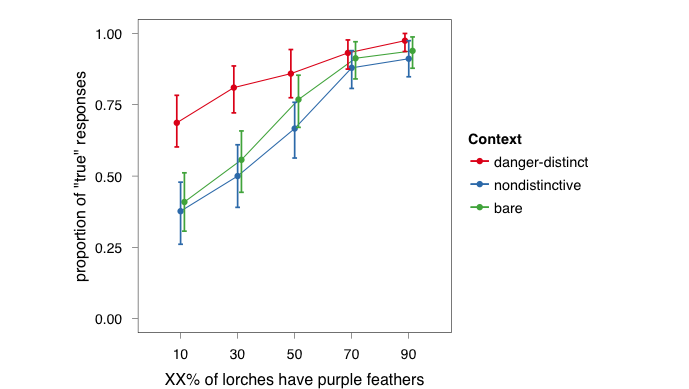
\includegraphics[width=\columnwidth]{fig1_replication}
%    \caption{Replication of CBG \emph{asymmetry}, generics condition}
%  \label{fig:replication}
%\end{figure}
%
We followed the data analysis strategy of CBG. Using the data from Exp. 1a, we computed, for each subject, an \emph{average prevalence level} that led to ``true'' responses (e.g. if a participant said ``true'' whenever the prevalence was 70\% or 90\% and ``false'' to everything else, that participant received an \emph{average prevalence score} of 80\%). This score was compared against the implied prevalence dependent measure of Exp. 1b. 

The prevalence scores were entered into a linear mixed model with a by-participant random effect of intercept; the fixed effects were context and task with an interaction term. Our results replicated the asymmetry finding of CBG that the generic statement was interpreted as having a higher prevalence than its truth conditions would imply (i.e. main effect of task; $t(105.8) = 6.632; p < 0.001$; see Fig.~\ref{fig:datasym}).

\section{Fixed-threshold semantics}
The above results, replicated from CBG, indirectly constrain the truth conditions that participants are effectively using for generic statements within these experimental conditions. In this section we explore these truth conditions more directly using Bayesian data analytic techniques.
%
We first assume that the conditions for truth of the generic can be usefully represented by a threshold on prevalence: the generic is true when the prevalence of some property within a kind exceeds a given threshold (see \citeA{Cohen1999} for a similar assumption).


\subsection{A context-invariant fixed-semantics}
We first examine what this threshold would look like if it were invariant to context. 

\begin{align}
 g(x, \theta) = \begin{cases}
   1 & \text{if } x > \theta \\
   0       & \text{if } x \leq \theta
  \end{cases}
%  \tag{\theequation}
   \label{eq:ftsem}
\end{align}

%\begin{equation*}
%X(\omega) = \begin{cases}
%1 &\text{se $\omega\in A$}\\
%1250 &\text{se $\omega \in A^c$}
%\end{cases}



%\citeA{Cohen1999} began his analysis by positing $\theta = 0.5$. A glance at the replication data in Figure \ref{fig:exp1} casts doubt on this assumption: there doesn't seem to be anything magical about 50\%. 
Here, $x$ is the proportion of a kind within a property (i.e. $x \in [0,1]$). How must $\theta$ be set to account for the data observed? 
To begin our data analysis, we make no \emph{a priori} assumptions about $\theta$, placing on it a uniform prior distribution: $\theta \thicksim U(0,1)$. 
We account for inattention and other irrelevant factors by including a probability $\phi_{t}\thicksim U(0,1)$ for each task\footnote{Ideally, we would have $\phi$ be a function of participant (some participants guess more than others) and experimental condition (some conditions are more difficult or less constrained and invite more guessing). This is computationally too demanding when coupled with the more complex cognitive model explored later.} that a given response is the result of uniform random guessing\footnote{What exactly \emph{random guessing} would mean in the case of the \emph{implied prevalence} task is unclear. For practical purposes, we considered there to be ten salient numbers between 0 and 100 (the tens), and thus guessing was selecting a particular response with a $\frac{1}{10}$ probability.} \cite{LW2014}.
The inferred ``guessing'' parameter $\phi$ is the amount of data that would have to be attributed to random guessing in order for the fixed-threshold model of the generic to apply to the experimental data. In this sense, $\phi$ gives a coarse notion of fit. 
We analyze the data from Exp. 1a and 1b jointly as well as independently.


%Following standard practice in Bayesian data analysis \cite{LW2014}, we include the data-analytic parameter $\phi$ to account for data points that deviate strongly from our theory; it is a guessing parameter. We assume there is some proportion of responses where the participant is responding randomly, and we estimate this quantity by way of $\phi$. We model two such $\phi$ parameters, one for each task.
%
%\begin{align*}
%\theta \thicksim U(0,1) \\
%\phi_{t} \thicksim U(0,1) %\mid  t \in \{exp1a, exp1b\}
%\end{align*}


%We formalize the notion of ``effective truth conditions'' by saying the generic is a function from states of the world to truth-values. We operationalize \emph{states of the world} here as the prevalence of some property within a kind. This mapping is then determined by some threshold such that the generic is true when the prevalence is above threshold. 

%Using the Church probabilistic programming language to represent this model \cite{probmods}, this would be written:
%
%\begin{lstlisting}
%(define generic 
%	(lambda (prevalence) (> prevalence generic-threshold)))
%\end{lstlisting}

%To handle the inference problem the participant is faced with, we express the subject's uncertainty about whether the generic is true or false.
%
%\red{NDG: the rest of this section is too long and doesn't make sense to me...}
% \begin{lstlisting}
%(define truth-conditions (lambda (prevalence)
%	(query  
%	
%		(define generic ...) ;defined as above
%		(define generic-is-true? (flip 0.5))
%		
%		generic-is-true?
%			
%		(generic prevalence))))
%\end{lstlisting}



%\subsubsection{Inferred parameters}



The joint analysis using a context-invariant semantics produces almost meaningless results. The inferred $\phi_{1a}$ is near 1 and the inferred $\theta$ is also near 1 (the $\phi_{1b}$ has a more reasonable posterior mean of 0.3). The joint analysis discounts the \emph{truth conditions} data entirely and uses only the \emph{implied prevalence} data to set the threshold, which results in a very high inferred threshold. (Recall that the \emph{implied prevalence} task alone suggests the generic is interpreted as a universal quantifier.)

The by-experiment analysis produces more interpretable results consistent with the overall theme of CBG. The implied threshold $\theta$ of the generic is completely different for the two tasks. For the implied prevalence task, the threshold is at least 90 and may be as high as 99. For the truth conditions task, the threshold is probably\footnote{This uncertainty results from the sparseness of our sampling (see Procedures and Materials). Participants were queried only at prevalence levels 10, 30, 50, 70, and 90} greater than 10\% and less than 30\%, however there is some non-zero probability that the threshold is in fact 0\%. 

The amount of guessing for the \emph{truth conditions} task ($\phi_{1a}$) is no longer near 1, but is still quite high, around 0.5, which means that participants would have to be guessing 50\% of the time. Though this analysis shows an asymmetry between the two tasks, it doesn't have the ability to capture the context-dependence present in the data. 
%we already know there is an effect of context on the generic meaning. There is no way for this model to account for such data.

%\begin{figure}
%\centering
%    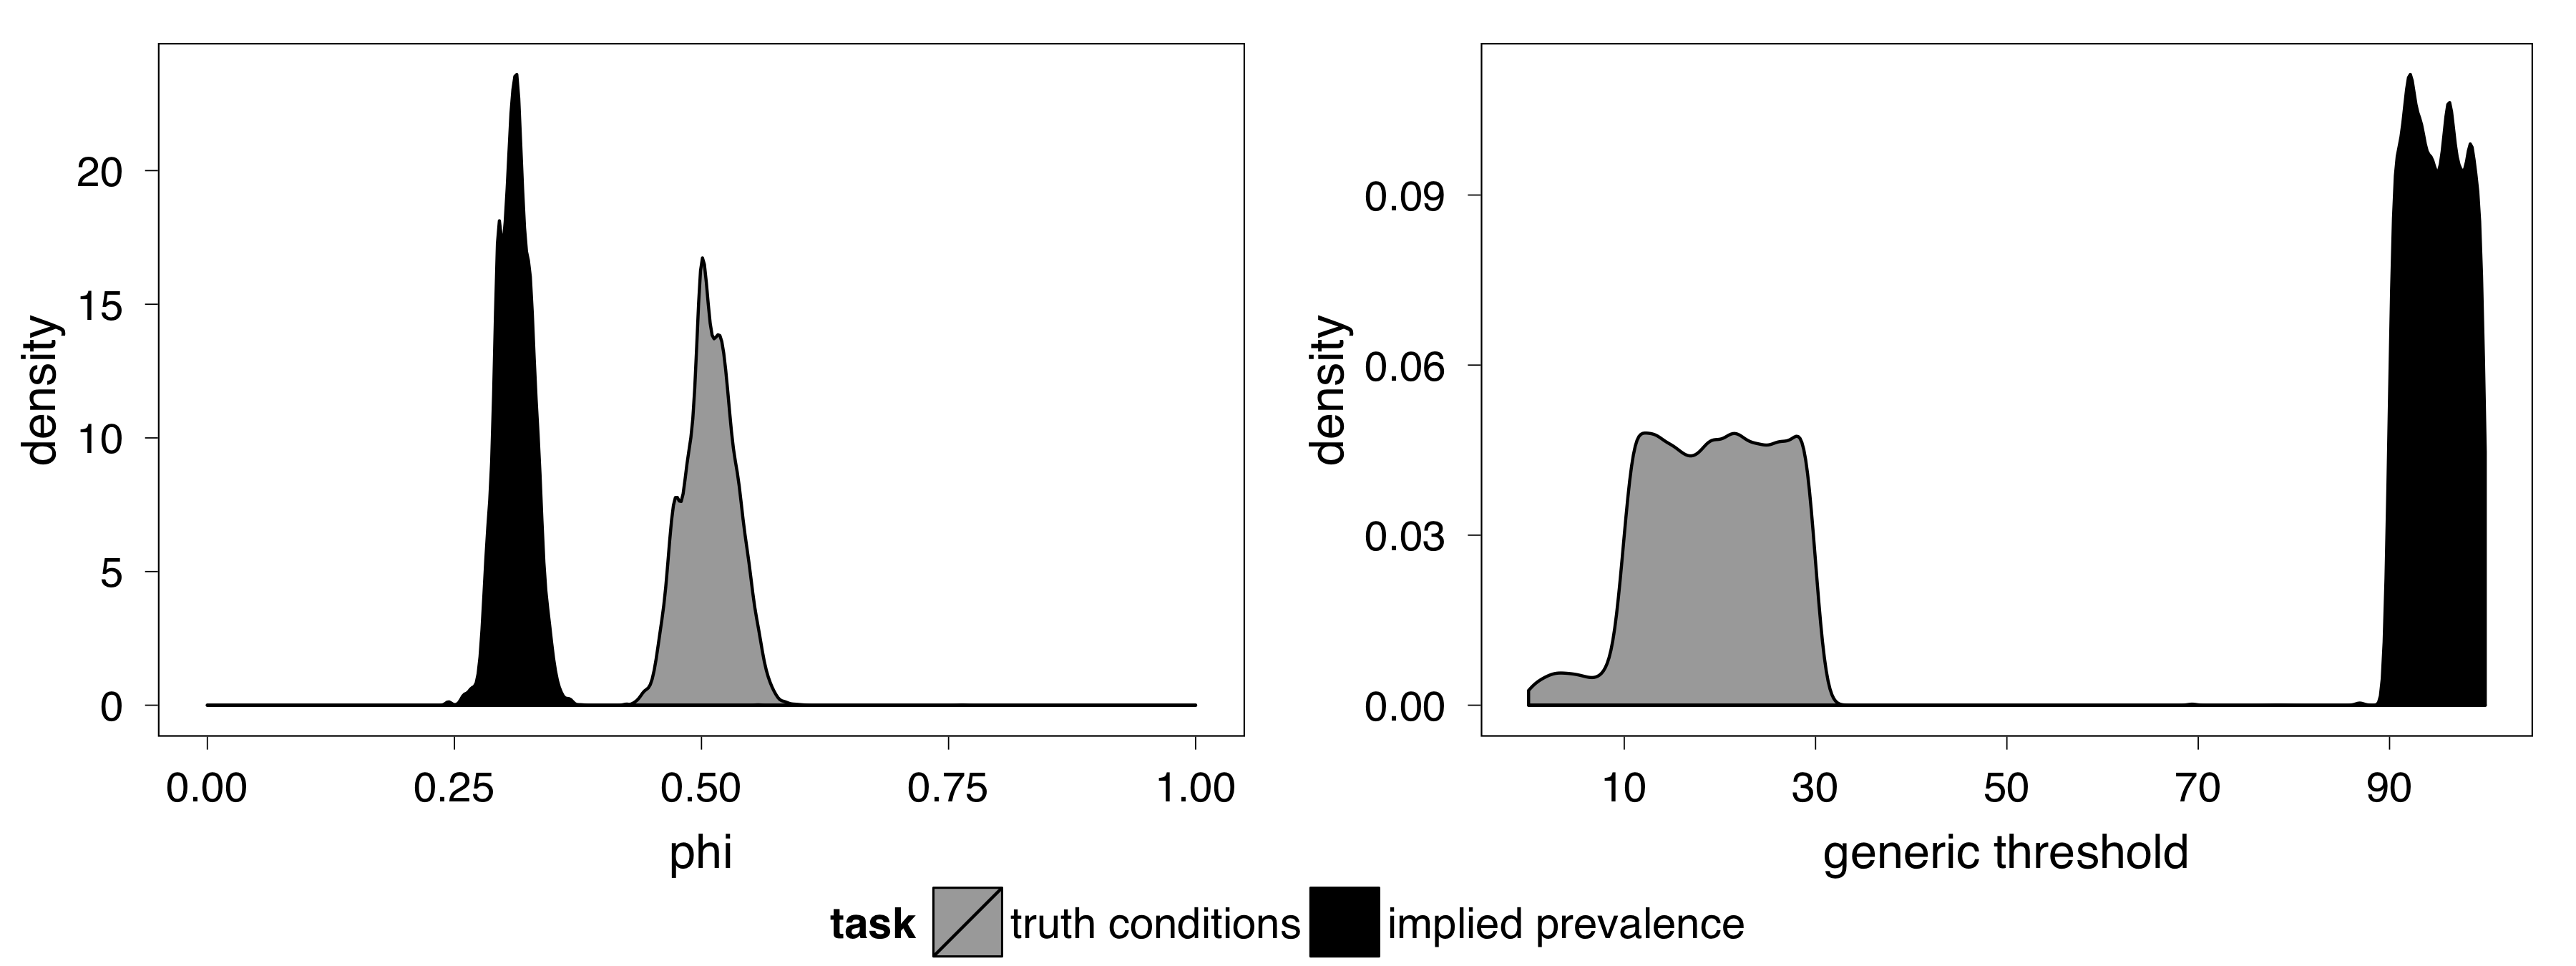
\includegraphics[width=\columnwidth]{trulyFixed_phis_thetas}
%    \caption{Fixed and context-invariant semantics of a generic. Inferred ``guessing'' parameter (left) and threshold (right) for each experiment.}
%  \label{fig:trulyfixed}
%\end{figure}


\subsection{A context-dependent fixed-semantics}

In Exp. 1a, we replicated CBG's evidence that the generic truth conditions vary by context. We reexamine our fixed-semantics model, now allowing for the possibility that $\theta$ could vary by context: $g(x,\theta_{c})$.
Again, we put uniform priors over each of the $\theta_{c}$'s. We are now in a position to ask how the truth-functional threshold of the generic behaves across these three contexts. 

%\subsubsection{Inferred parameters}

The results can be seen in Figure \ref{fig:justFixed}. The first observation is that there is indeed variability in the generic threshold, at least in the \emph{truth conditions} task. In the \emph{plain} condition, the analysis suggests the threshold is somewhere between 0\% and 30\%, but it's unclear where exactly in that range the threshold should be. Critically, in the \emph{dangerous and distinctive} context, the analysis infers a lower threshold, less than 10\%. This matches with the earlier Null Hypothesis analysis. Finally, and most intriguingly, the analysis infers a third distinct threshold profile for the \emph{irrelevant and nondistinct} context.  The inferred threshold is greater than 10\%, but could be as high as 50\%. This is an overall higher inferred threshold for the nondistinctive category; however, these results are inconclusive as to whether or not this threshold is different from the \emph{plain} context.

\begin{figure}
\centering
    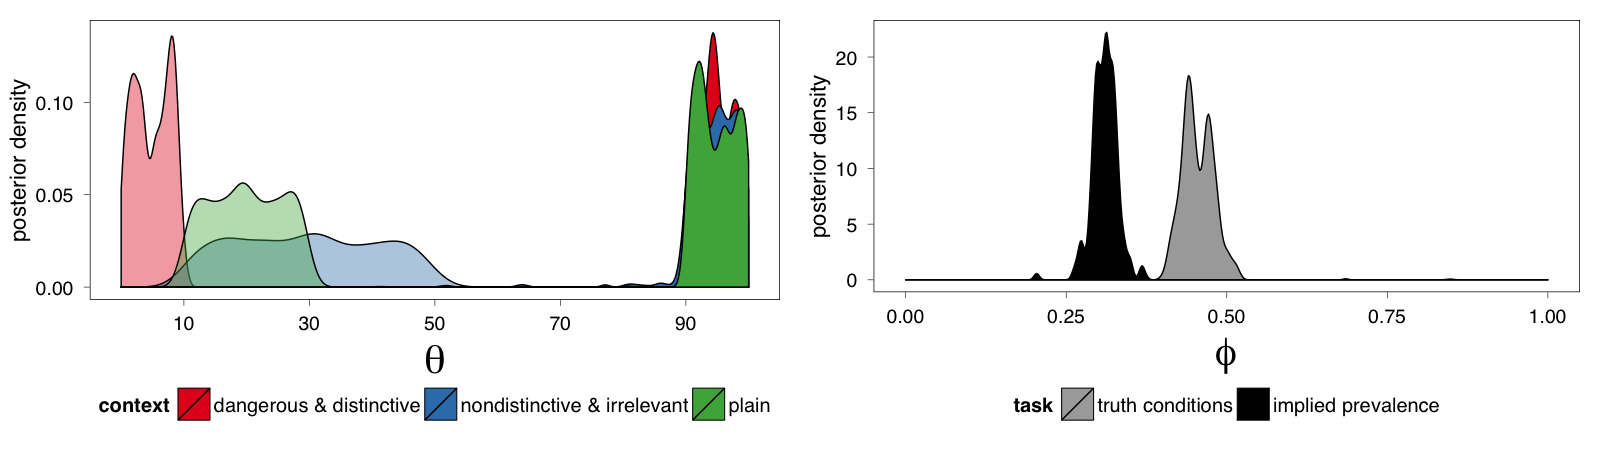
\includegraphics[width=\columnwidth]{fixed_phis_thetas}
    \caption{Fixed and context-sensitive semantics of a generic. Inferred ``guessing'' parameter (left) and threshold (right) for each experiment.}
  \label{fig:justFixed}
\end{figure}

The posterior distribution for $\phi_{t}$'s shows a marginal improvement over the context-invariant semantics for the \emph{truth conditions} task (posterior mean $\thicksim 0.45$). Still, however, the amount of data that must be attributed to guessing to be consistent with this model of generics is quite high.
%\subsubsection{Posterior predictives}

The inflexibility of the model can also be seen in the posterior predictive distribution of responses. 
The posterior predictive distribution marginalizes over the inferred parameter values to produce predictions about what the data should look like given the cognitive model and the observed data. This is akin to fitting the parameters and is an important step in model validation as it shows what data the model actually predicts.
%\footnote{As a thought experiment, consider 2 coins assumed to come from a single coin-making machine (all the coins from this machine have the same weight). You flip each coin 100 times. The first one returns 100 heads, and the second one returns 100 tails. The posterior mean of the inferred coin weight will be 0.5. Comparing the posterior predictive distribution (based on this inferred coin-weight) to the observed data, however, will highlight the fact that your theory about the ``single coin-making machine'' is seriously flawed.}.
Following directly from the inferred $\theta_{c}$'s, the model matches the ordering of the truth-conditions by context reasonably well. However, each prediction curve is a step-function and is too dichotomous to match the human data. The correlation between the posterior predictive and the data is $r = 0.81$. 

The fixed-threshold semantics model is not flexible enough to explain the observed data, but it has an even more serious flaw: the variation of threshold by condition is postulated \emph{a priori} in the data analysis, rather than accounted for by the cognitive model. That is, participants in our experiment must have some way of arriving at different thresholds for different tasks and conditions, which this model has no means to explain. For a more explanatory model we turn to the pragmatics of language understanding.


%\begin{itemize}
%\item Inferred value of theta across contexts. 
%\item $\phi$ parameter. 
%\item Posterior predictive of fixed threshold model?
%The problem with this approach is that we are assuming there is some threshold for the generic, out there in the world, and that all there is to do is go out and measure it. An alternative is to consider that there is indefeasible uncertainty about the threshold, but that listeners try their best and actively infer, from context, probable values of the threshold. To express this type of model, we must consider the pragmatics of language understanding. 


%A \lstinline{query} is a special function in Church. The first arguments to a query function are a generative model: definitions or the background knowledge with which a reasoning agent is endowed. Definitions for which a random choice is stipulated (e.g. \lstinline{(define generic-is-true? (flip 0.5))}) denote aspects of the world over which the agent has uncertainty. The second argument, called the \emph{query expression}, is the aspect of the computation that the model should return. The final argument, called the \emph{conditioner}, is the information with which the agent updates beliefs. 
%
%This is the simplest model of the truth conditions of the generic. It says the subject has maximal uncertainty as to whether or not the generic is true (expressed by \lstinline{(flip 0.5)}, a Bernoulli random variable). The subject uses the prevalence given to her to determine if the generic is true. 
%
%At the same time, we want to take into account the results of Exp. 1b: the interpretation of the generic. Here, we are concerned with the interpretation of the utterance, so we put uncertainty over the prevalence. We condition on the fact that the generic must be true of the prevalence, whatever it may turn out to be.
%
% \begin{lstlisting}
%(define implied-prevalence (lambda (utterance)
%	(query  
%		
%		(define generic ...) ;defined as above
%		(define prevalence (uniform 0 1))
%		
%		prevalence
%			
%		(generic prevalence))))
%\end{lstlisting}
%
%We are now in a position to ask how the truth-functional threshold of the generic behaves across these three contexts. To do this, put each of these models inside of a Bayesian data analysis model. The data analysis model posits that \lstinline{generic-threshold} might be a function of context.
%
%The data analysis model can be written very simply in Church.
%
%\begin{lstlisting}
%(define bayesian-data-analysis 
%	(query
%		; we don't know the generic threshold but we feel it might be a function of context
%		(define generic-threshold 
%			(mem (lambda (context) (uniform 0 1))))
%		(define truth-conditions ...) ; defined as above
%		(define implied-prevalence ...)
%		
%		(define phi (uniform 0 1)); guessing parameter
%				
%		generic-threshold ; return generic-threshold	
%		
%		(and 
%			(= experiment1a-data truth-conditions)
%			(= experiment1b-data implied-prevalence))))
%
%\end{lstlisting}
%
%The model above is a data analysis model to try to infer the threshold of the generic, with the built-in flexibility that it might vary by context. The functions \lstinline{truth-conditions} and \lstinline{implied-prevalence} jointly form our cognitive theory\footnote{This could be made more explicit by moving the function \lstinline{generic} outside of either \lstinline{query}, since it is the same function. This function is the core of this cognitive theory.}. It says the generic is like an alien quantifier. This quantifier behaves like other quantifiers in that it has a fixed-threshold semantics. The only thing special about the generic is that the threshold might be different for different contexts. 
%
%We don't know what the generic might mean \emph{a priori}. Thus, the generic-threshold\footnote{If the generic threshold turns out to be 0, the generic ``Lorches have purple feathers'' would mean essentially, ``Some lorches have purple feathers''. If the threshold turned out to be very close to 1, the generic would mean essentially: ``All lorches have purple feathers''.} follows a uniform prior distribution between 0 and 1. 
%
%The \lstinline{query} function is written to return \lstinline{generic-threshold}, which is the parameter we are interested in inferring. Finally, the last line is our condition statement: we condition on the data we collected in Exp. 1a being explained by the \lstinline{truth-conditions} model and Exp. 1b to be explained by \lstinline{implied-prevalence}. For clarity, we have omitted the impact of \lstinline{phi}, but it comes into play in the condition statement. In reality, each response could have been generated by our theory (via \lstinline{truth-conditions} or \lstinline{implied-prevalence}) or by guessing (via \lstinline{phi}).  


%\end{itemize}

\section{Reasoning about the threshold}

%CBG showed how contexts affects the endorsement for generic statements. An additional concern of their experiments surrounded the relation between two dependent measures for understanding generics. One dependent measure was the ``truth conditions'', or \emph{sentence verification} measure that we've been considering up to this point. The other was an ``implied prevalence'', or \emph{sentence interpretation} dependent measure. The latter was collected by giving participants the generic statement (plus, any additional contextual information), and asking the participant ``What percentage of lorches have purple feathers?''

The tasks in Exp.~1 are, fundamentally, language understanding tasks. We draw on recent work from probabilistic pragmatics to formalize our intuitions about how listeners arrive at interpretations of utterances. In particular, we draw on work from the Rational Speech Act (RSA) theory of language understanding. In this framework, a listener infers the meaning of an utterance by a recursive reasoning process, wherein the listener considers the thought-processes of a speaker whose goal is to be informative. Variants of this theory have provided computational explanations for a number of linguistic phenomena including scalar implicature, hyperbole, and multiple classes of reasoning paradigms \cite{Kao2014, Tessler2014, Lassiter2014}. 

%\subsection{Lifted-variable RSA}

%The Bayesian data analysis above provides compelling evidence that context influences the truth-conditions of a generic statement. The poor qualitative fit as well as the high inferred value of the guessing parameter $\phi$ suggest, however, that our language model is incomplete. Rather than propose that the meaning of a generic is simply a one-to-one mapping between context and threshold, 

We propose that the literal semantics of a generic sentence is in fact a threshold on prevalence, but listeners don't know the appropriate threshold and actively reason about it in context. 
A similar proposal has been made to explain gradable adjectives like \emph{tall}. 
\citeA{Lassiter2015}  propose the meaning of an adjective like \emph{tall} is a standard truth-functional meaning such that the object in question \emph{is tall} if it has a height greater than the threshold $\theta_{tall}$. 
The vagueness and context-sensitivity of scalar adjectives are accounted for by treating $\theta_{tall}$ as an unknown property of the language, and modeling the pragmatic listener as inferring this threshold.
 
%The key insight, though, is that the listener has uncertainty about what $\theta_{tall}$ actually is, and infers that value of $\theta_{tall}$ via the same recursive reasoning process through which she infers the intended meaning of the utterance.

%How is a listener supposed to reason about $\theta_{tall}$? In the case of adjectives, reasonable thresholds are inferred by way of the prior distribution of the property in question. ``John is tall'' and the ``Empire State Building is tall'' imply different heights for John and the ESB because the prior distributions of heights for people and buildings are different. An adjective will only be informative (and truthful) with respect to the appropriate prior distribution. 



%In Church, the model looks like:
%
%\begin{lstlisting}
%(define pragmatic-listener (lambda (utterance)
%	(query
%		(define prevalence (prevalence-prior))
%		; listener doesn't know the threshold
%		(define generic-threshold (threshold-prior))
%			
%		prevalence
%			
%		(equal? utterance 
%		; listener imagines the speaker does know the threshold
%			(speaker prevalence generic-threshold)))))
%			
%(define speaker (lambda (prevalence generic-threshold)
%	(query
%		(define utterance (utterance-prior))
%			
%		utterance
%			
%		; speaker conditions on a literal-listener inferring the right prevalence
%		(equal? prevalence 
%			(literal-listener utterance generic-threshold)))))
%			
%(define literal-listener (lambda (utterance generic-threshold)
%	(query
%		(define prevalence (prevalence-prior))
%			
%		prevalence
%		; literal listener conditions on the words being true
%		(utterance prevalence generic-threshold))))
%\end{lstlisting}

The RSA model for generic interpretation, with the prevalence threshold as a variable ``lifted'' to pragmatic reasoning is specified by:
\begin{flalign}
& P_{L_{0}}(x \mid g, \theta) \propto g(x, \theta) P(x) \label{eq:L0} \\
& P_{S_{1}}(g \mid x, \theta) \propto \exp{(\alpha \ln{P_{L_{0}}(x \mid g, \theta)})} \label{eq:S1}\\
& P_{L_{1}}(x , \theta \mid g) \propto P_{S_{1}}(g \mid x, \theta) P(x) \label{eq:L1}
\end{flalign}
The literal content of the generic in Eq.~\eqref{eq:L0} is identical to the fixed-threshold model in Eq.~\eqref{eq:ftsem}. However, it interacts with the prior distribution $P(x)$ over prevalence levels---the prior distribution of prevalence of a particular property across kinds.

Eq.~\eqref{eq:L1} is a model of a listener ($L_{1}$) who has been told a generic statement. She assumes that, whatever the speaker ($S_{1}$) meant to communicate, the speaker was trying to be informative and that his goal was to communicate the prevalence $x$. She assumes the speaker in Eq.~\eqref{eq:S1} knows $\theta$ and chooses an utterance to be informative to the literal listener ($L_{0}$).  From this, the listener jointly infers both $x$ and $\theta$. We call this type of model a ``lifted variable'' model (lvRSA) because $\theta$, traditionally thought to be part of the semantic content of the utterance (and thus perfectly transparent to all in the conversation), has been underspecified in the semantics but is locally fixed by pragmatic reasoning.

The prevalence prior $P(x)$ has a critical effect on the interpretation of the generic in this model. As a simplification, we posit a family of possible priors $x \thicksim \beta(\gamma,\delta)$\footnote{For ease of interpretation, we are parametrizing the $\beta$ distribution by its mean and concentration. To recover the canonical shape parametrization, use $\gamma \delta$ and $(1-\gamma)\delta$.}. We hypothesize that the details of this prior (i.e.~$\gamma$ and $\delta$) may differ according to the context in which a generic is used. For instance, when you know that a particular property is rare, a different distribution over categories is called to mind, than if the property is common. This results in different meanings for the generic. Below we infer appropriate prior parameters for each context from the behavioral data.

Following the advice of \citeA{Degen2014}, who investigated the relationship between dependent measures and speaker and listener roles in RSA, we will model the \emph{implied prevalence} task as a pragmatic listener ($L_{1}$) task, but the \emph{truth conditions} task as a pragmatic speaker task. We model the truth judgment with a speaker $S_{2}$ who is trying to convey the prevalence to a pragmatic listener, but can only produce the generic or its negation (i.e.~yes or no to the truth of the generic):
\begin{equation} 
P_{S_{2}}(g \mid x) \propto \exp{(\alpha \ln{P_{L_{1}}(x \mid g) P(g)})}.
\label{eq:S2}
\end{equation}
The speaker in \eqref{eq:S2}, like $L_{1}$, doesn't know the threshold, but knows that $L_{1}$ is thinking about it, and marginalizes over possible values: $ P_{L_{1}}(x \mid g) = \sum_{\theta} P_{L_{1}}(x , \theta \mid g) $.


%\begin{lstlisting}
%(define lifted-speaker (lambda (prevalence)
%	(query
%		(define utterance (utterance-prior))
%			
%		utterance
%			
%		(equal? prevalence (pragmatic-listener utterance)))))	
%\end{lstlisting}


%\subsection{Bayesian analysis to infer priors}


%\begin{lstlisting}
%(define bayesian-data-analysis
%	(query
%	
%		(define gamma ; mean prevalence
%			(lambda (context) (uniform 0 1)))
%			
%		(define delta ; concentration of our distribution around the mean
%			(lambda (context) (uniform 0 5)))
%			
%		(define phi (uniform 0 1)) ; guessing parameter
%	
%		(define lifted-speaker ...) ; lvRSA model
%		(define pragmatic-listener ...)
%		(define speaker ...)
%		(define literal-listener ...)
%				
%		'(gamma delta)
%				
%		(and 
%			(= experiment1a-data lifted-speaker)
%			(= experiment1b-data pragmatic-listener))))
%\end{lstlisting}

%\begin{figure}
%\centering
%    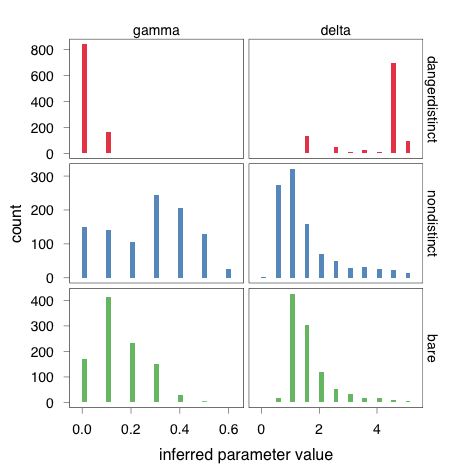
\includegraphics[width=\columnwidth]{fig4_bda2_hyper}
%    \caption{Hyperprior parameters for lifted-variable RSA model}
%  \label{fig:bda2hyperparams}
%\end{figure}

\subsection{Results}

We again do a Bayesian data analysis to evaluate this more sophisticated cognitive model. We are interested in how the hyperprior parameters $\gamma$ and $\delta$ might vary across contexts.
We put uncertainty over the parameters of the prevalence prior, $\beta(\gamma,\delta)$, outside of the RSA cognitive model (but inside of the data analysis model). 
\begin{align*}
\gamma_{c} \thicksim U(0,1) \\
\delta_{c} \thicksim U(0,5) \\
\phi_{t} \thicksim U(0,1) 
\end{align*}
Here, $c \in \{DD,NI,P\}$ and $t \in \{$truth conditions, implied prevalence$\}$.
We keep the data-analytic guessing parameters $\phi_{t}$ as a gross estimate of the proportion of responses our model of cognition doesn't capture. 



%We propose that, in this paradigm, nobody knows $\theta$.  $\theta$ is influenced by the prior distribution over prevalence, which in turn is influenced by the contextual information provided (\emph{DD}, \emph{NI}, or \emph{P}). This contextual information could imply different $P(x)$, prior probability distributions over the prevalence of a property. 
%
%Naively, this distribution would be $U(0,1)$, or equivalently, $\beta(1,1)$. However, we propose that people have different prior distributions in mind, depending on features of the properties under discussion (e.g. distinctiveness).
%
%Although we might have some intuitions what these prior distributions might look like, we put uncertainty over the parameters of this Beta distribution $\beta(\gamma,\delta)$, outside of the RSA model but inside of the data analysis model. 
%
%\begin{align*}
%x_{c} \thicksim \beta(\gamma_{c},\delta_{c}) \\
%\gamma_{c} \thicksim U(0,1) \\
%\delta_{c} \thicksim U(0,5) \\
%\phi_{t} \thicksim U(0,1) 
%\end{align*}
%
%Here, $c \in \{DD,NI,P\}$ and $t \in \{$truth conditions, implied prevalence$\}$.
%
%Thus, we do Bayesian data analysis on a Bayesian Rational Speech-Act model of language understanding, to see how context might influence the prior distribution given the data we've observed. We keep the data-analytic guessing parameters $\phi_{t}$ as a gross estimate of the proportion of responses our model of cognition doesn't capture. 

\subsubsection{Inferred parameters}
The mean inferred values of  $\phi_{1a}$ and $\phi_{1b}$ are about 0.08 and 0.05, respectively, a seemingly reasonable\footnote{Without proper control tasks, it's impossible to know what proportion of guessing to expect. Here, we are assuming Turkers are cooperative and so lower values for $\phi_{t}$ are better.} estimation of ``guessing'' probability for participants on Amazon's Mechanical Turk, indicating that this cognitive model is doing a much better job of accounting for participants' responses.

%We use Bayesian data analysis to infer the values of the hyperprior parameters $\gamma$ and $\delta$ for the Bayesian lvRSA model. 
Figure \ref{fig:posthyper} shows the posterior distributions of the hyperprior parameters, $\gamma$ and $\delta$, for the lvRSA model. The posterior means for the $\gamma$'s (the $\beta$ mean parameter) are well-ordered: $DD < P < NI$. This can be directly interpreted as the mean prior prevalence for the three contexts: \emph{dangerous and distinctive} properties are more rare than the other two types of properties. The posterior means for the $\delta$'s (the $\beta$ concentration parameter) are also ordered, suggesting greater uncertainty about the $P$ context than about the other 2. 


\begin{wrapfigure}{l}{0.5\columnwidth}
  \begin{center}
    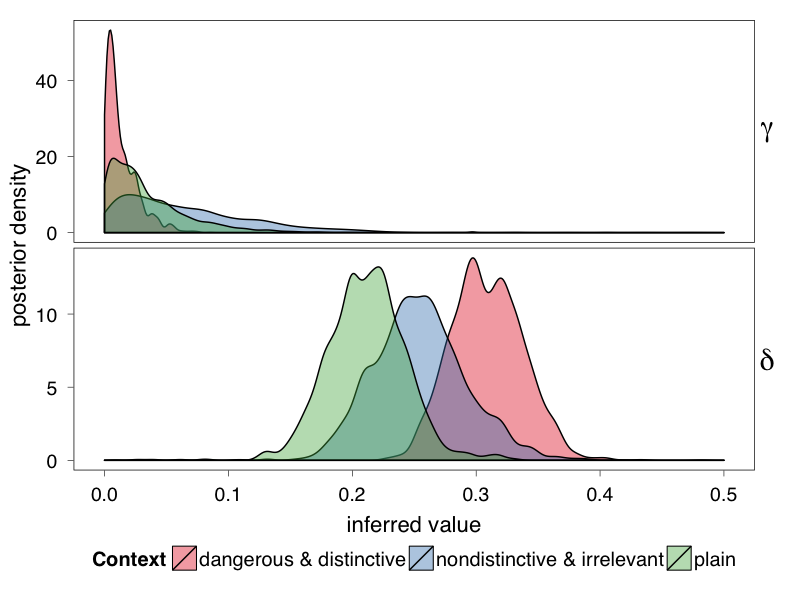
\includegraphics[width=0.48\columnwidth]{inferred_hyperpriors}
  \end{center}
  \caption{Posterior distributions of the hyperprior parameters used in lvRSA.}
   \label{fig:posthyper}
\end{wrapfigure}


%\begin{wrapfigure}{r}{0.5\textwidth}
%%\centering
%   \begin{center}
%    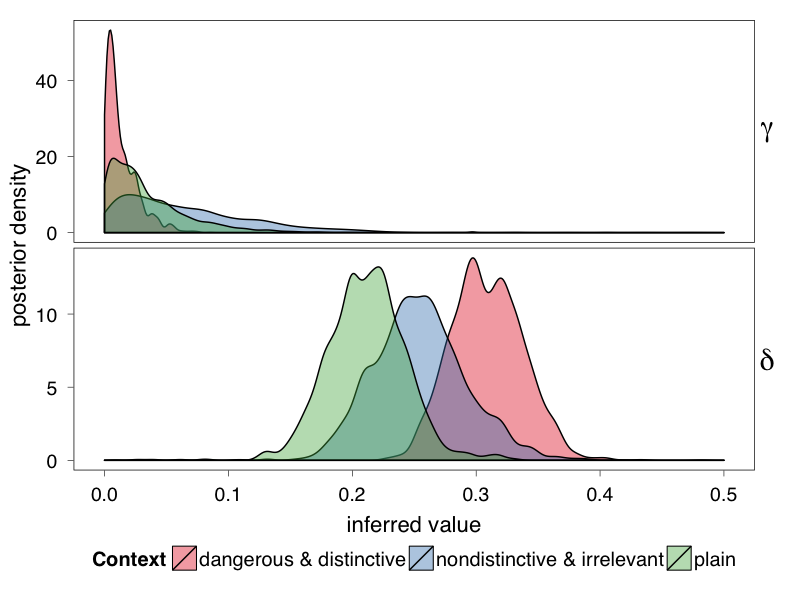
\includegraphics[width=0.48\columnwidth]{inferred_hyperpriors}
%    \end{center}
%    \caption{Posterior distributions of the hyperprior parameters used in lvRSA.}
%  \label{fig:posthyper}
%\end{wrapfigure}

%begin{table}[h]
%\centering
%\begin{tabular}{c | c | c}
%context / parameter & $\gamma$ & $\delta$ \\
%\hline
%DD                  & 0.016  & 0.321  \\
%NI                  & 0.054  & 0.245  \\
%P                   & 0.031  & 0.204 
%\end{tabular}
%\caption{Posterior means for hyperprior parameters.}
%\label{table:postmeans}
%\end{table}
%

For further visualization, we marginalize over the posterior parameter values to reconstruct a canonical prior distribution over prevalence for each context. Figure \ref{fig:inferredpriors} shows these prior distributions inferred from Exp. 1a \& 1b data via the lvRSA model. 

\subsubsection{Posterior predictives}


The posterior predictions by lvRSA for the \emph{truth conditions} task are in Figure \ref{fig:lvRSAposteriorpred}. 
We can see that the model predicts graded endorsement rates for the generic as a function of prevalence---the model has some persistent uncertainty about the true value of the threshold, a feature that people share.
With the inferred parameter values of the prevalence prior, the model also matches the differences in endorsement rates between context conditions.
We reconstruct the curves of Figure \ref{fig:exp1} well; the model--data correlation is $r = 0.90$.

%lvRSA models the \emph{truth conditions} task as a speaker---$S_{2}$ using Eq.~\eqref{eq:S2}---faced with the task of saying whether or not the generic applies to a given prevalence of a property. This utterance is intended for a pragmatic listener---$L_{1}$ using Eq.~\eqref{eq:L1}---who will try to reconstruct the prevalence that $S_{2}$ has observed. Here, we have modeled the \emph{implied prevalence} task as this listener, $L_{1}$, given the utterance, tasked with reconstructing the prevalence. 

We use a similar data analysis strategy as we did for Exp. 1b to compare ``average prevalence'' between verification and interpretation. For the \emph{truth conditions} data, we took the model's posterior probability of saying ``true'' at each prevalence level. We normalized these posterior probabilities so they added to 1. We then took the inner product of these probabilities and the prevalence levels to compute an ``average prevalence'' score for the model. Since $L1$ returns a posterior distribution over prevalences, we could use the \emph{implied prevalence} data directly. We find the model predicts the asymmetry between interpretation and verification of the generic (see Figure \ref{fig:lvRSAposteriorpred}, right).

%\subsubsection{Discussion}

\begin{figure}
\centering
    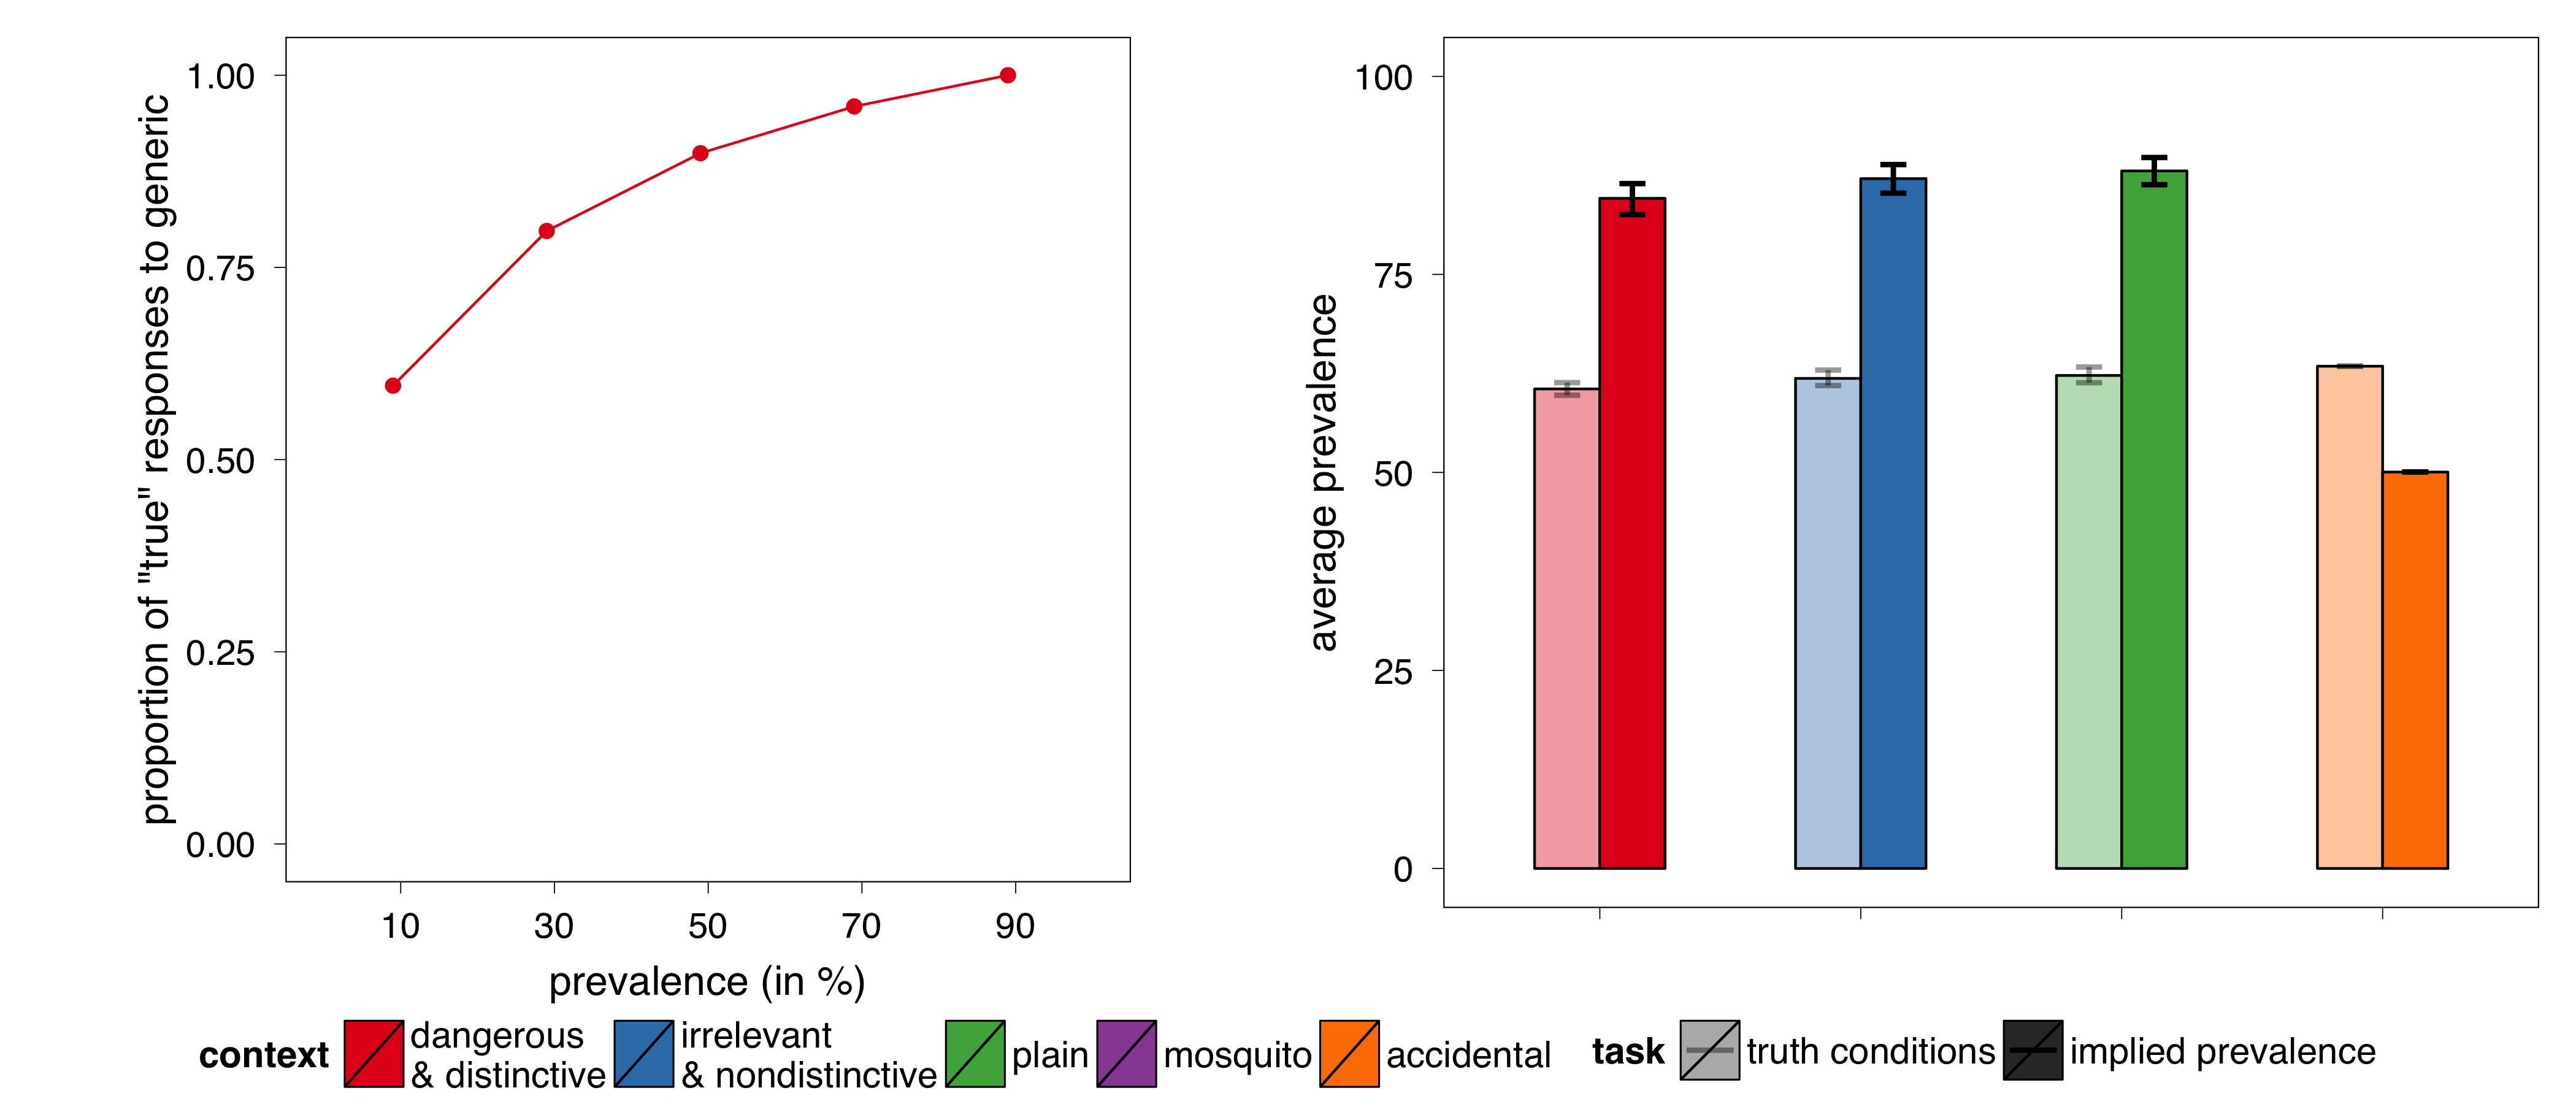
\includegraphics[width=\columnwidth]{lvRSA_postpreds_wSims}
    \caption{Posterior predictives of lvRSA for truth conditions (left) and asymmetry between dependent measures (right). Mosquitos and Accidental predictions use schematic priors (see text).}
  \label{fig:lvRSAposteriorpred}
\end{figure}


To see how this asymmetry is possible, consider again the inferred prevalence priors in Figure \ref{fig:inferredpriors}. They are bimodal with peaks around 0\% and 100\%. This is consistent with the intuition that biological properties, such as the ones used by CBG, are properties either held by all of a category or none of category. Since the semantics of the generic is underspecified (i.e. $\theta$ ---the threshold of endorsement for truth judgement--- is unknown), if $\theta$ falls anywhere in the range between 10\%-90\%, the most likely prevalence is going to be near 100\%. Hence, in the \emph{implied prevalence task}, the most likely inferred prevalence could be appreciably higher than one would expect from the \emph{truth conditions} task. 




%\begin{figure}
%\centering
%    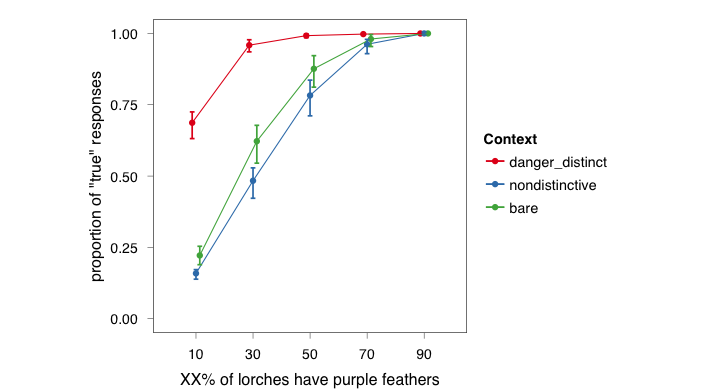
\includegraphics[width=\columnwidth]{fig5_bda2_postpred}
%    \caption{Posterior predictive using lifted-variable RSA}
%  \label{fig:postpred2}
%\end{figure}

Often in Bayesian data analysis, the posterior distribution over parameters is hard to interpret in terms of observable phenomena. Our case is more transparent: if lvRSA were the correct model in this task, the prior distributions of prevalence for the three contexts should look like they do in Figure \ref{fig:inferredpriors}. 
In particular, all three types of properties should have bimodal prior prevalence distributions, with a high probability that 0\% of the kind have the property. Further, this left skew should be more pronounced for the \emph{DD} properties relative to the \emph{P} properties. 

\section{Experiment 2}

\begin{figure}
        \centering
        \begin{subfigure}[b]{\columnwidth}
    			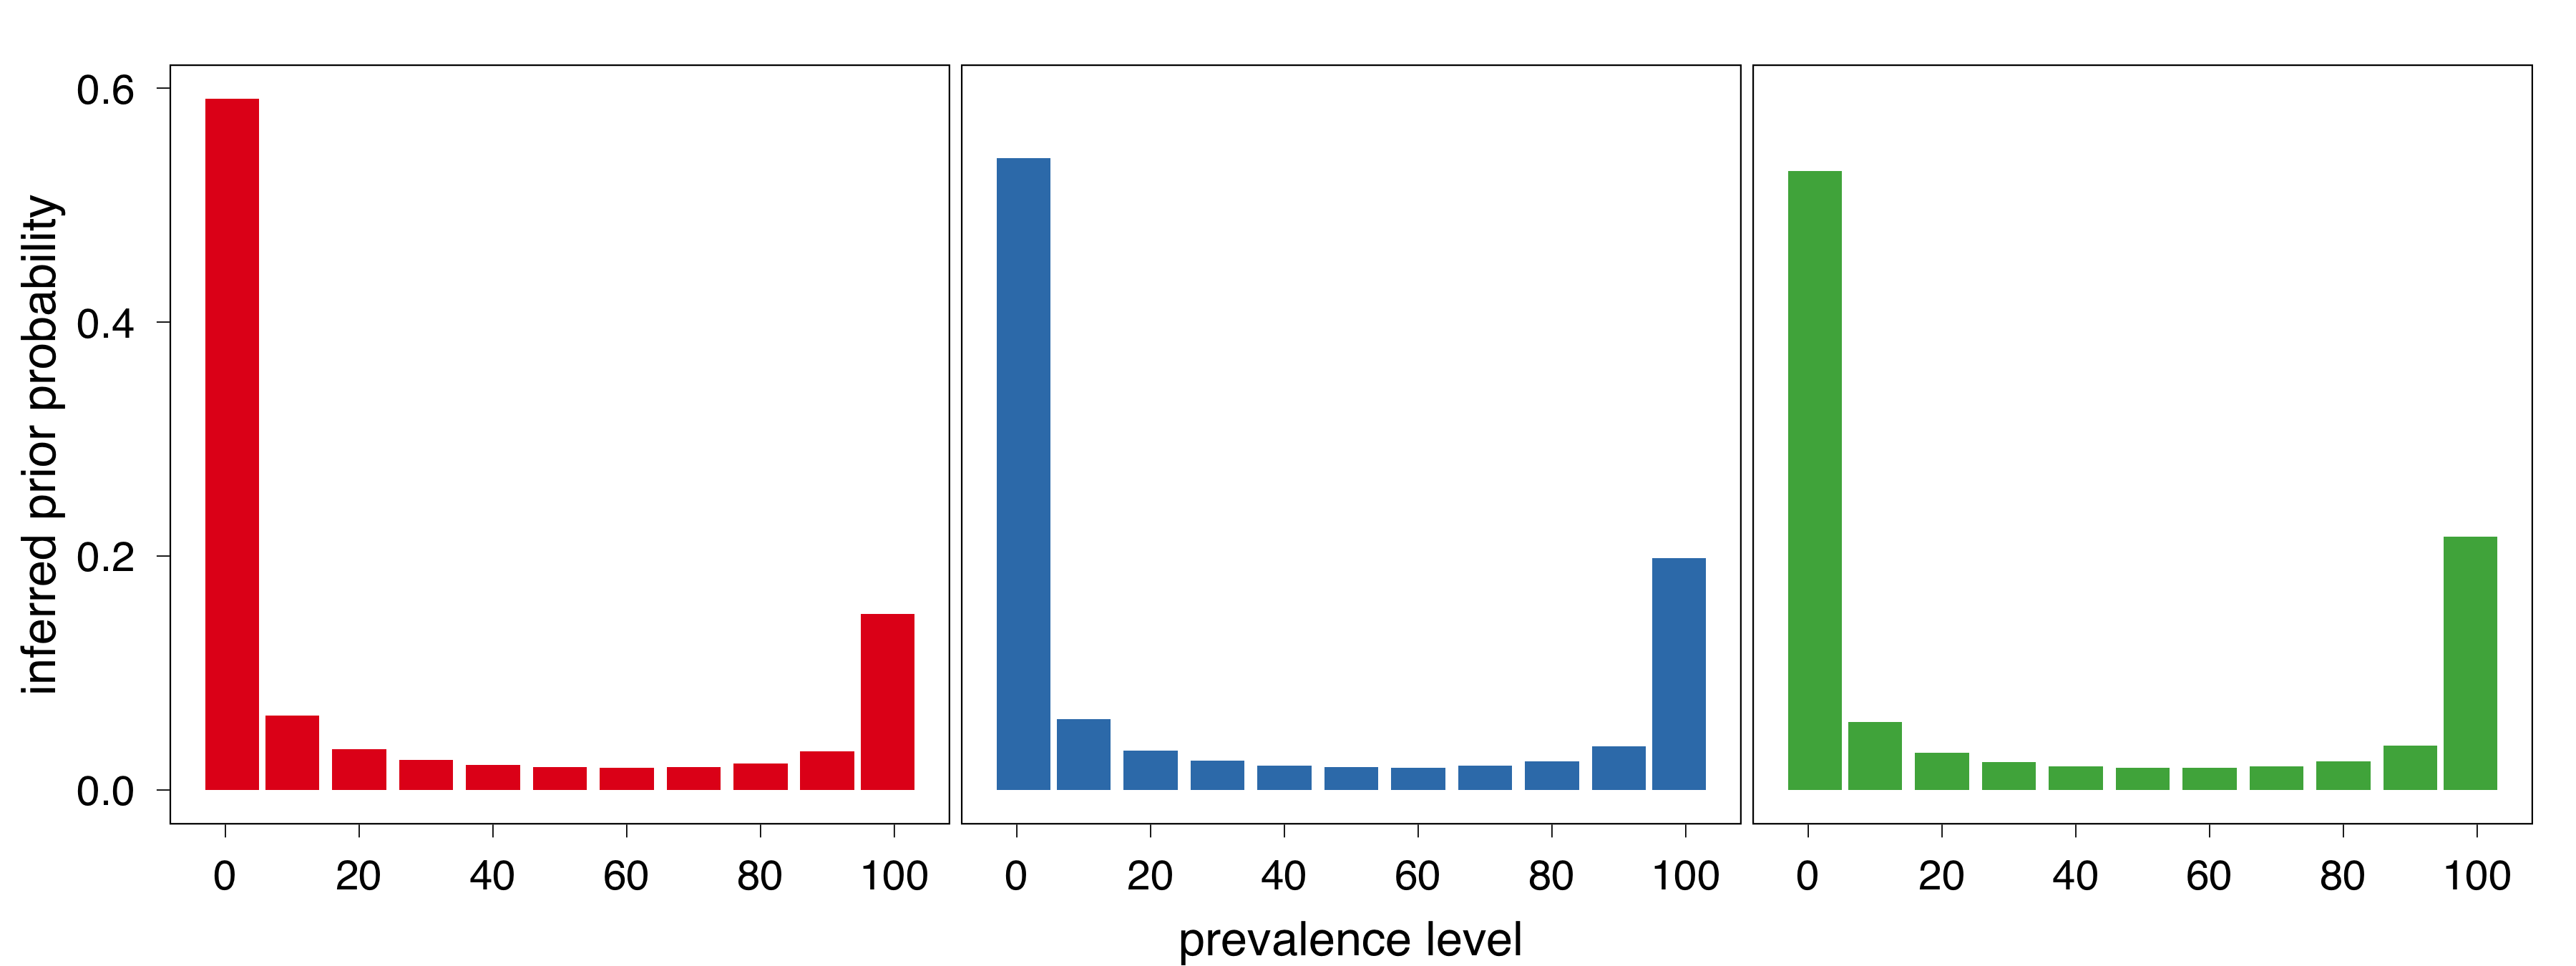
\includegraphics[width=\columnwidth]{inferred_marginalized_priors}
                \caption{Reconstructed priors from marginalized posterior $\gamma$ and $\delta$, for each context.}
                \label{fig:inferredpriors}
        \end{subfigure}%
        
        ~ %add desired spacing between images, e. g. ~, \quad, \qquad, \hfill etc.
          %(or a blank line to force the subfigure onto a new line)
        
        \begin{subfigure}[b]{\columnwidth}
                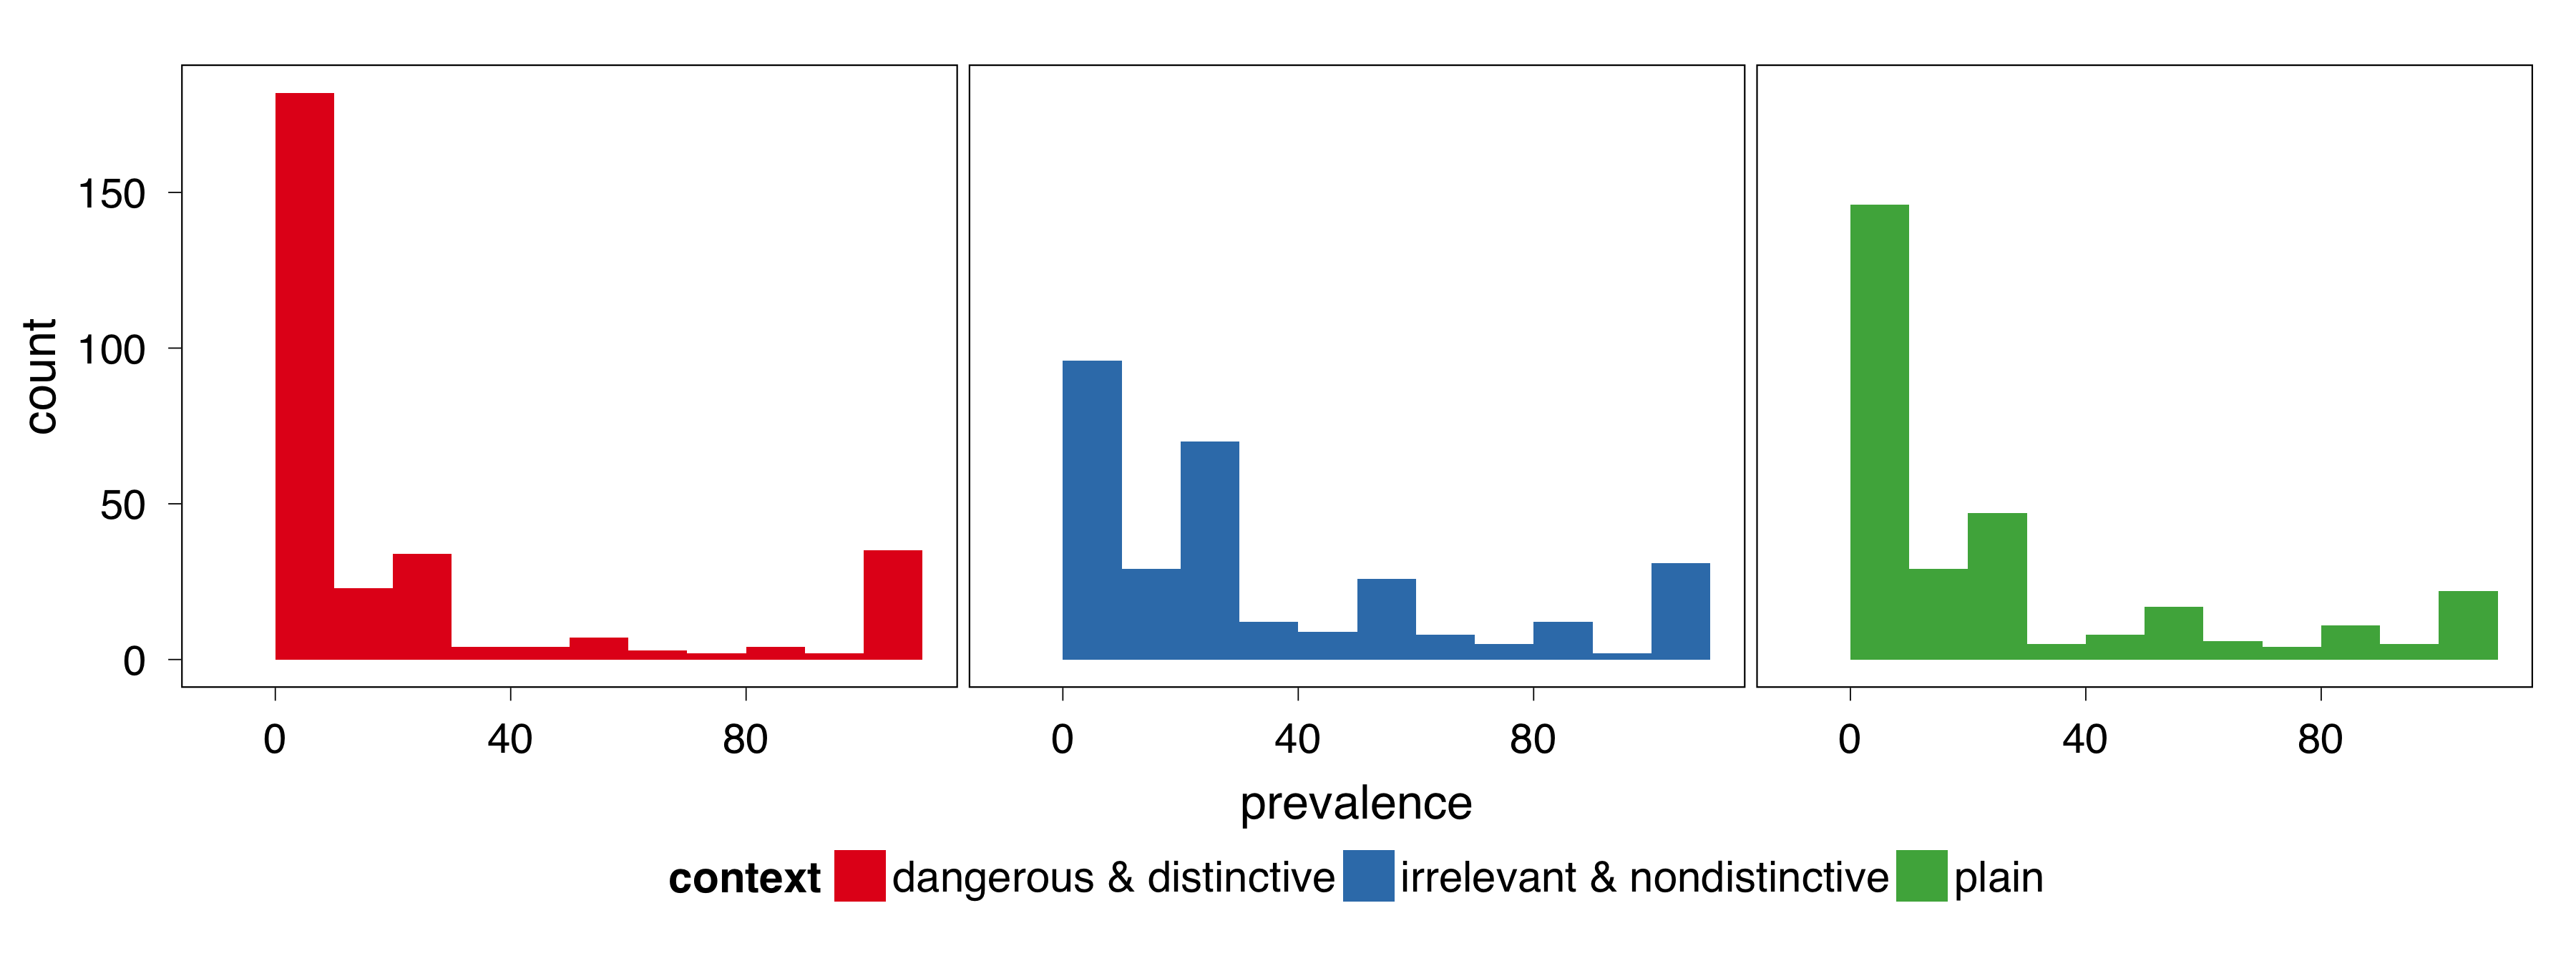
\includegraphics[width=\columnwidth]{elicited_priors}
                \caption{Priors elicited in Experiment 2.}
                \label{fig:elicitedpriors}
        \end{subfigure}
        ~ %add desired spacing between images, e. g. ~, \quad, \qquad, \hfill etc.
          %(or a blank line to force the subfigure onto a new line)
        \caption{Prior distributions over prevalence.}\label{fig:priors}
\end{figure}


Exp. 2 sought to test the prediction that the prior distribution of prevalence levels would be bimodal and vary by context.

\subsection{Method}

\subsubsection{Participants}

We recruited 30 participants over Amazon's crowd-sourcing platform Mechanical Turk. 

\subsubsection{Procedure and materials}

Our procedure\footnote{The experiment in full can be viewed at \url{http://stanford.edu/~mtessler/experiments/generics/cbg2010-replication/experiment/experiment-11.html}} was similar to Exp. 1b. On each trial, participants either read contextual information (\emph{DD} or \emph{NI}) or nothing (\emph{plain}). 

In addition to the contextual information, participants were presented with the following: ``Listed below are 5 kinds of animals, recently discovered.'' and asked the following question: ``What percentage of each kind of animal do you think has [property]?'' The experiment consisted of 6 trials, 2 from each context. 

\subsubsection{Results}

Experiment 2 recovered the shape of the inferred prior distributions from the lvRSA model (compare Figure \ref{fig:elicitedpriors} to Figure \ref{fig:inferredpriors}). Hartigans' Dip Test for Unimodality is highly significant for each of the prior distributions ($D = 0.055, 0.0667, 0.045$ for contexts $DD, NI, P$, respectively; p < 0.0001 for each), and thus the distributions are at least bimodal. The correlation between these probabilities is $r = 0.90$.

\section{Discussion}

We have demonstrated the viability of a scalar semantics for generics within an RSA framework. The lower-bound threshold on the prevalence of the property in the category is inferred as part of pragmatic interpretation, yielding vague and context sensitive meaning. We first used Bayesian data analysis to show that the effective threshold of a fixed-threshold semantics would need to vary by context, and yet it still not account adequately for the data. We then formalized pragmatic reasoning about the threshold in a lifted-variable Rational Speech Acts (lvRSA) model. This model predicted graded truth judgements and an asymmetry between truth and prevalence judgements. It also accommodated the context, explaining these effects as the result of variation in the prevalence prior. In Experiment 2, we verified that participants' beliefs about the prior on prevalence varied in this way. Over all, this provides evidence that the model we propose can account for many of the puzzling aspects of generic meaning.

%We have shown how a Bayesian model of language understanding, motivated by contextual variation of the effective threshold of the generic statement, can explain the puzzling truth conditions and asymmetrical meanings of generic language. We have used techniques in Bayesian data analysis to help arbitrate between two cognitive theories. The first was a simple theory that proposed that a generic was akin to some alien quantifier. In this theory, the generic behaves like other quantifiers in that it has a fixed-threshold semantics. We explored one elaboration of this in allowing the generic to have a threshold that differed across contexts. 
%
%The alternative theory is that there is no generic threshold out there in the world to observe. Instead, listeners infer the threshold (and thus, the semantic content) of the words from context. The posterior predictive distributions of the lvRSA model account for the contextual variation in the generic endorsements, both quantitatively and qualitiative. It further accounts for the asymmetry between verification and interpretation by considering different Questions Under Discussion (QUDs) and communicative roles (speaker / listener) in the two tasks. Finally, the Bayesian analytic techniques allowed us to make a new prediction as to the shape of the prior distribution over prevalence levels for different contexts. Exp. 2 found confirmatory evidence that this is indeed how people think these properties are distributed.

%\section{Further simulations}
%
%Our model makes the prediction that if the shape of the prior distribution was not bimodal, the asymmetry between verification and interpretation would change. Indeed, this is a similar prediction to \citeA{Cimpian2010}, who posited that accidental or disease states (e.g. ``muddy feathers'', ``infected ears'') would weaken the asymmetry. We would expect accidental or disease states to not follow a bimodal distribution. 
 

This model of generic interpretation makes further predictions for situations in which the shape of the prevalence prior differed. For example, if the prior distribution was unimodal, as is the case with incidental properties (e.g. broken legs), then the asymmetry between verification and interpretation would be dramatically reduced, cease altogether, or reverse (see Figure \ref{fig:lvRSAposteriorpred} for a prediction using the schematic prior in Figure \ref{fig:schematic}). Indeed, CBG explored this possibility in one of their experiments using ``accidental and disease states''; consistent with lvRSA, they found no asymmetry. 
\begin{wrapfigure}{r}{0.5\columnwidth}
  \begin{center}
    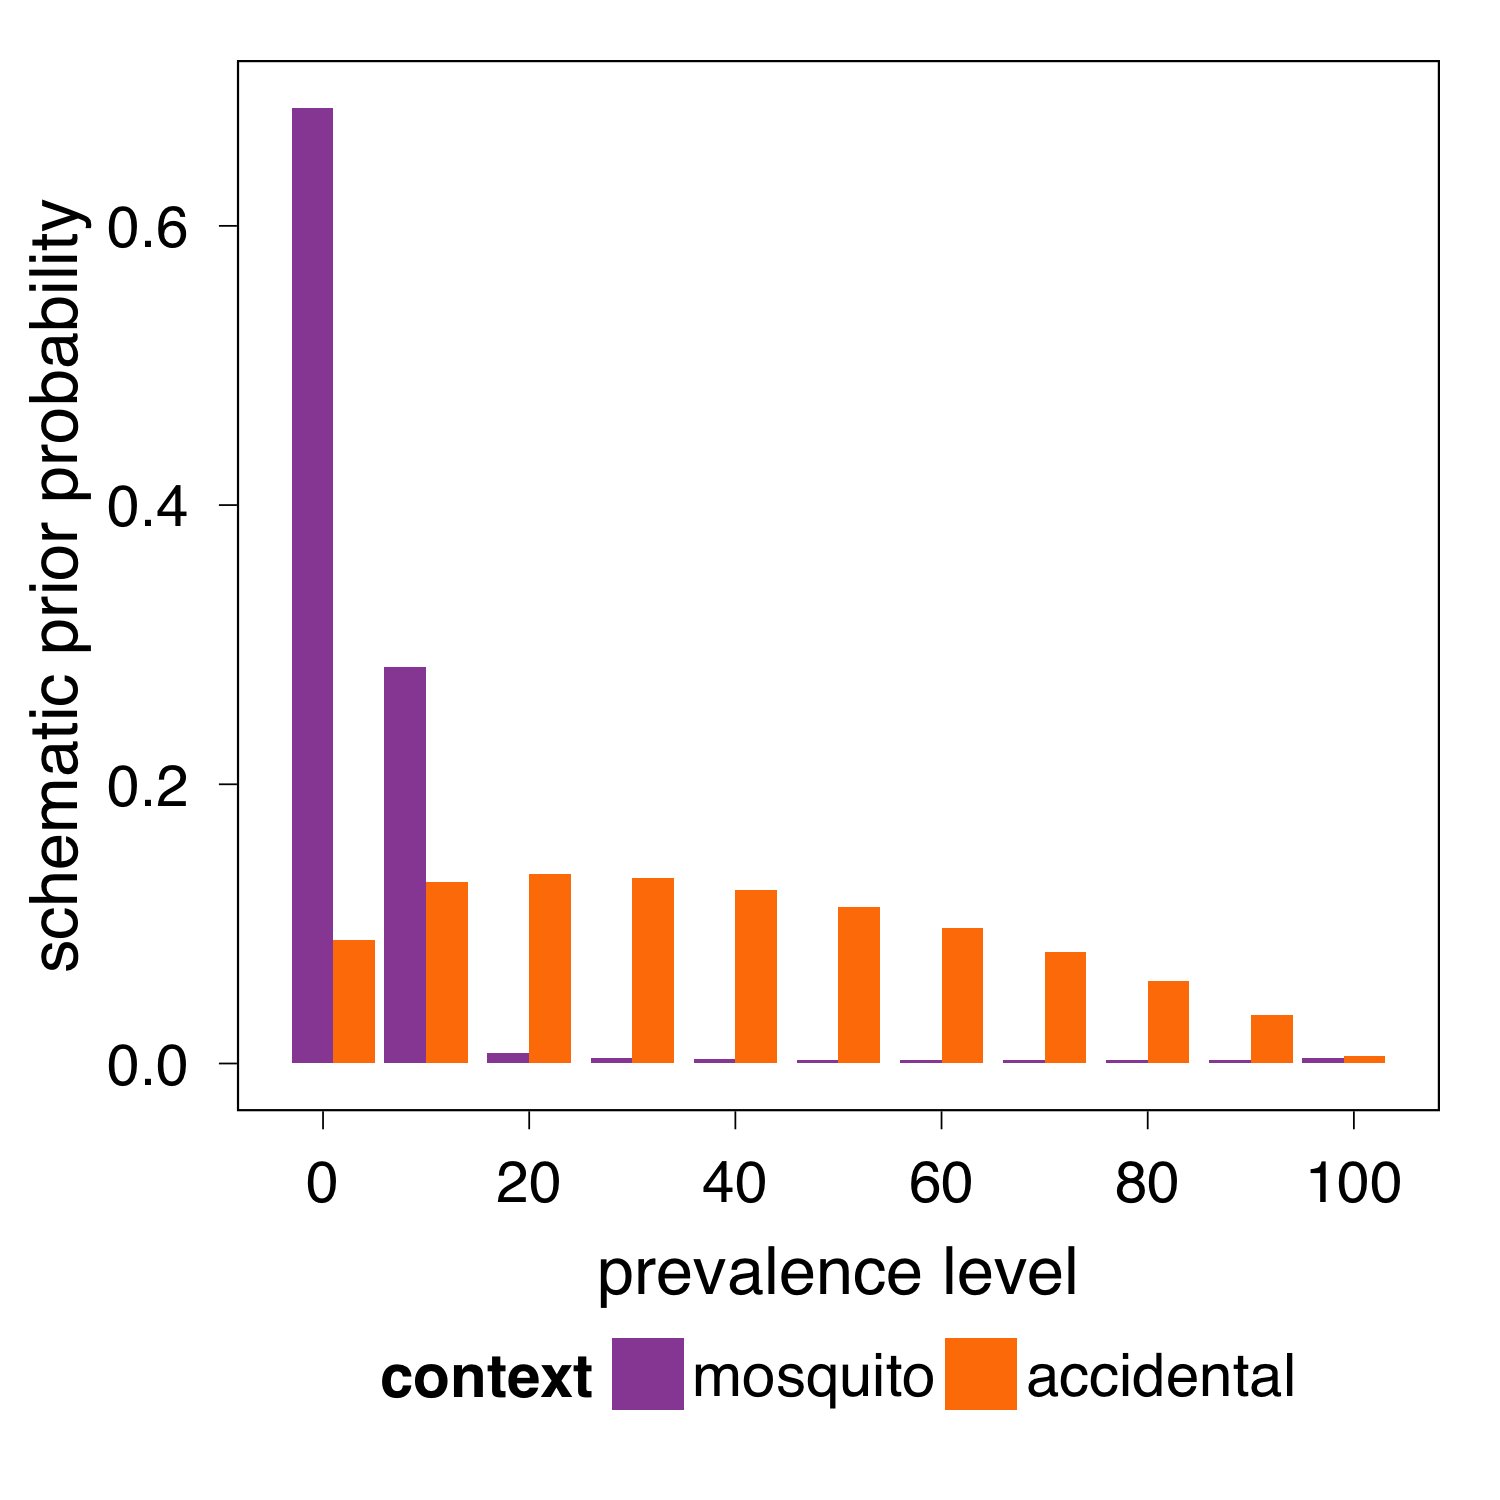
\includegraphics[width=0.48\columnwidth]{schematic_priors}
  \end{center}
  \caption{Schematic prior distributions over prevalence of accidental properties and ``mosquitos with West Nile Virus''.}
   \label{fig:schematic}
\end{wrapfigure}
%
Another example is a bimodal prior with a second peak at some low prevalence level (as opposed to a bimodal prior with a second peak at a high prevalence level, which we've focused on in this paper). This prior should describe rare properties that are not only rare \emph{across kinds} but also rare \emph{within kinds}. A canonical example of this is ``West Nile Virus'' in the generic ``Mosquitos carry West Nile Virus''. For a prior like this, the truth conditions for the generic would be relaxed at low prevalence levels, relative to the more common bimodal priors. We see this behavior using a schematic prior (see Figure \ref{fig:lvRSAposteriorpred} for the truth conditions of the mosquito prior shown in Figure \ref{fig:schematic}). 


Generics are ubiquitous in natural language. It might seem paradoxical, then, that the semantics of generic statements are underspecified. Why should vague language get so much usage? One possibility is apparent in the lvRSA model: generic language provides interlocutors with the flexibility to convey rich meanings, which are easily understood in context. 
Generics are vague, but principled and useful.

%In this paper, we used techniques of both Bayesian Cognitive Science and Bayesian Data Analysis. The former helped us develop a rich, formal theory of language understanding. These sorts of theories have implications for psychology and linguistics. The latter helped us make inferences about our theories. Bayesian Data Analysis is crucial to make assumptions explicit (e.g. about fixed-threshold semantics) and clean up our data (e.g. discounting behavior that can conceivably be attributed to guessing). Together, they embody a manifestation of a more general philosophy of science: making assumptions explicit and beginning our science by announcing our uncertainty.


%\begin{itemize}
%
%\item Replace figure 4 (hyperprior parameters) with mean distribution?
%
%\item Collapse Figure 3 \& 5 (posterior predictive) into one
%
%\item Exp 2 to confirm $\gamma$ and $\delta$. 
%
%\item Some linking function to condition on Exp 1 \& 2 simultaneously,  to perhaps, infer rationality parameter and get some posterior predictives.
%
%\end{itemize}
%
%The data analysis involved comparing the mean of the prevalence ratings associated with \emph{True} endorsements of the generic with the mean prevalence ratings elicited by the generic in a separate task. In the experimental pragmatics literature, the dependent measure involved in the ``truth conditions'' task is called \emph{sentence verification}; in the ``implied prevalence'' task, it is a \emph{sentence interpretation}. 
%
%These different dependent measures, we argue, imply different Questions Under Discussion (QUD, \cite{Roberts2004}). 



%	\section{Sentence verification is a speaker task}
%	
%	DegenGoodman2014.  Truth conditions task --> QUD = ``generic true?'' Model.
%	
%	But what is the semantics of the generic? \citeA{Cimpian2010}, experiments 1, 3, and 4 found that the truth conditions of the generic are sensitive to the context.  Our goal is to replicate this finding, and use Bayesian data analysis to infer the threshold of the speaker model. This bears some similarity to Michael Franke's approach for cogsci from last year.
%	
%	
%	
%	
%	\section{The full bayesian thing}
%	
%	Computational models of cognition typically have parameters. Many of these parameters are of theoretically interest, because they are posited to reside within the head of the subject.
%	
%	\subsection{Inferring quantifier threshold by context}
%	
%	Here we'll find that the generic threshold changes by context. We might also want to show that ``most'' and ``some'' do not change by context.
%	
%	\subsection{Are generics like adjectives?}
%	
%	To determine if a generic is true or false, we must refer to context. The threshold in the threshold-semantic view of the statement varies by context. This property has been shown to be an important feature in the semantics of gradable adjectives (e.g. \emph{tall}) \cite{Lassiter2014}.  
%	
%	\section{Lifted-variable speech act model}
%	
%	We can start in a single context, with a uniform prior over states. We can look at the posterior over states, for listener1. As well, we can look at the posterior over thetas. This depends of course on the alternatives, for which we may want to consider only the experimental alternatives \emph{some, most, generic} or for which we may want to include \emph{all}.  Either way, here we'll recreate the asymmetry between listener and speaker --- between implied prevalence and truth conditions. 
%	
%	\citeA{Cimpian2010} report a ``paradoxical asymmetry at the core of generic meaning'' which manifests as the generic having ``extremely strong implications but requiring little evidence to be judged true''. Here, we explain this ``paradox'' by the different Questions Under Discussions in the tasks used and by the different roles intrinsic to speech-acts: the role of the speaker and the role of the listener. 
%	
%	\subsection{Questions Under Discussion in two tasks}
%	
%	\citeA{Cimpian2010} used two tasks (with different dependent measures) to get at the comparison between ``acceptance'' and ``implications''. These two tasks --- called ``truth conditions'' and ``implied prevalence'' -- used different questions and different dependent measures to get at the meaning of generics. In the ``truth conditions'' task, subjects are given evidence about the prevalence of a property (e.g. ``50\% of morseths have silver fur'') and are asked to judge the corresponding generic (i.e. ``Morseths have silver fur'') to be either true or false. In the ``implied prevalence'' task, subjects are given a generic statement and asked ``What percentage of morseths do you think have silver fur?''
%	
%	\citeA{Degen2014} argue that the \emph{sentence verification} (``truth conditions'') task should be modeled as a speaker task, and that the \emph{sentence interpretation} (``implied prevalence'') task should be modeled as a listener task. In addition to different communicative roles, there are also different implicit Questions Under Discusision. In the ``truth conditions'' task, the QUD seems to be ``is the generic true or false?'', whereas in the ``implied prevalence'' task, the QUD seems to be ``what percentage of category X have property Y?''.





\bibliographystyle{apacite}

\setlength{\bibleftmargin}{.125in}
\setlength{\bibindent}{-\bibleftmargin}

\bibliography{generics}


\end{document}


% after cogsci
% prior elicitation for accidental / disease states
% -- asymmetry weakened

% most / some: better experiments
% -- asymmetry X prior analysis

